\documentclass[tikz,border=5pt]{standalone}

\usepackage{pgfplots}
\pgfplotsset{compat=1.18}

\begin{document}

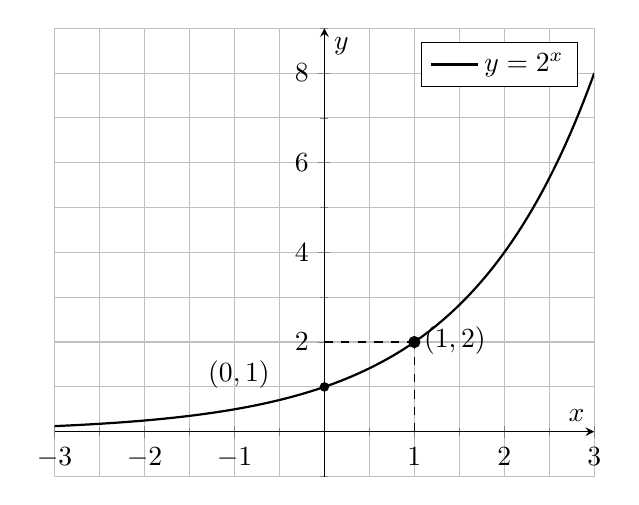
\begin{tikzpicture}
  \begin{axis}[
      axis lines = middle,
      xmin = -3, xmax = 3,
      ymin = -1, ymax = 9,
      samples = 200,
      xlabel = {$x$},
      ylabel = {$y$},
      grid = both,
      minor tick num = 1,
      domain = -3:3,
      legend style={at={(0.97,0.97)},anchor=north east},
    ]

    % Plot y = 2^x
    \addplot[thick] {2^x};
    \addlegendentry{$y = 2^x$}

    % Emphasize the point (1, 2)
    \addplot[
      only marks,
      mark=*,
      mark size=2pt
    ] coordinates {(1,2)};

    % Dashed helper lines to the axes
    \addplot[dashed] coordinates {(1,0) (1,2)};
    \addplot[dashed] coordinates {(0,2) (1,2)};

    % Label the point (moved up and right so it doesn't sit on the curve)
    \node[above right] at (axis cs:1,1.5)
      {$(1,2)$};

    % Emphasize the y-intercept at x = 0
    \addplot[
      only marks,
      mark=*,
      mark size=1.5pt
    ] coordinates {(0,1)};

    % Label the y-intercept (moved left and up)
    \node[above left] at (axis cs:-0.5,0.75)
      {$(0,1)$};

  \end{axis}
\end{tikzpicture}

\end{document}
